%Authors guidlines: http://royalsocietypublishing.org/instructions-authors
% 2500 words max (includes the title page, abstract, references, acknowledgements and figure/table legends)
% current version is around 3700. I think a big cut down can be done on the references.
% We allow a maximum of 4 displays, only 2 of which can be figures.

\documentclass[12pt,letterpaper]{article}
\usepackage{natbib}

%Packages
\usepackage{pdflscape}
\usepackage{fixltx2e}
\usepackage{textcomp}
\usepackage{fullpage}
\usepackage{float}
\usepackage{latexsym}
\usepackage{url}
\usepackage{epsfig}
\usepackage{graphicx}
\usepackage{amssymb}
\usepackage{amsmath}
\usepackage{bm}
\usepackage{array}
\usepackage[version=3]{mhchem}
\usepackage{ifthen}
\usepackage{caption}
\usepackage{hyperref}
\usepackage{amsthm}
\usepackage{amstext}
\usepackage{enumerate}
\usepackage[osf]{mathpazo}
\usepackage{dcolumn}
\usepackage{lineno}
\usepackage{longtable}
\pagenumbering{arabic}


%Pagination style and stuff % NC: Note that these are all syst biol specific.
\linespread{2}
\raggedright
\setlength{\parindent}{0.5in}
\setcounter{secnumdepth}{0} 
\renewcommand{\section}[1]{%
\bigskip
\begin{center}
\begin{Large}
\normalfont\scshape #1
\medskip
\end{Large}
\end{center}}
\renewcommand{\subsection}[1]{%
\bigskip
\begin{center}
\begin{large}
\normalfont\itshape #1
\end{large}
\end{center}}
\renewcommand{\subsubsection}[1]{%
\vspace{2ex}
\noindent
\textit{#1.}---}
\renewcommand{\tableofcontents}{}
%\bibpunct{(}{)}{;}{a}{}{,}

%---------------------------------------------
%
%       START
%
%---------------------------------------------

\begin{document}

%Running head
\begin{flushright}
Version dated: \today
\end{flushright}
\bigskip
\noindent RH: Morphological data availability in living mammals

\bigskip
\medskip
\begin{center}

\noindent{\Large \bf Morphological data is lacking for living mammals}
%Or: Missing cladistic data in living mammals - but I prefer the first one emphasizing on the availability of it. The data is not missing per se, it's just not coded!
% NC: sometimes the better title is one that answers the question rather than giving the topic. e.g., "Morphological data is lacking for living species" or similar
% TG: maybe worth considering the special issue as well? "Putting fossils in tree" so maybe something like "There is not enough morphological data for living mammals to branch fossils in the trees."
% TG: or some poetic... "Living and dead mammals: morphological data is lacking in living for combined analysis"

%Key words: Total Evidence method, data structure, phylogenetic, living, fossil, topology
\bigskip

\noindent {\normalsize \sc Thomas Guillerme$^1$$^,$$^2$$^,$$^*$ and Natalie Cooper$^1$$^,$$^2$$^,$$^3$}\\
\noindent {\small \it 
$^1$School of Natural Sciences, Trinity College Dublin, Dublin 2, Ireland.\\
$^2$Trinity Centre for Biodiversity Research, Trinity College Dublin, Dublin 2, Ireland.\\
$^3$Department of Life Sciences, Natural History Museum, Cromwell Road, London, SW7 5BD, UK.}\\
\end{center}
\medskip
\noindent{*\bf Corresponding author.} \textit{Zoology Building, Trinity College Dublin, Dublin 2, Ireland; E-mail: guillert@tcd.ie; Fax: +353 1 6778094; Tel: +353 1 896 2571.}\\  
\vspace{1in}

%Line numbering
\modulolinenumbers[1]
\linenumbers

%---------------------------------------------
%
%       ABSTRACT
%
%---------------------------------------------
% NC: I've commented this out so I don't have to keep scrolling past in in the PDF
%\newpage
%\begin{abstract} % 200 words, all keywords written in abstract if possible.
%Studying changes in global biodiversity through time and space is essential.
%For that we need methods to combine both palaeontological and neontological data.
%One promising method, the Total Evidence method, allows such thing but needs a lot of data.
%Especially cladistic data from living taxa to allow the fossil taxa to accurately branch in the trees.
%Despite two centuries of morphological studies on living taxa, scientists using and generating such data mainly focus on palaeontological data.
%Therefore, even in well known groups such as mammal, there is a huge gap in our knowledge of cladistic data for living mammals.
%In this study, using phylogenetic community structure methods, we quantify the availability of data in each mammalian order.
%And maybe at the end of the paper we propose some discussion on how to improve all that (go in museums!).
%\end{abstract}

%\noindent ()\\

%\vspace{1.5in}

%---------------------------------------------
%
%       INTRODUCTION
%
%---------------------------------------------

%NC: I've changed cladistic to morphological throughout but you might want to change it back...

\newpage 
\section{Introduction}
There is an increasing consensus among evolutionary biologists that studying both living and fossil taxa is essential for fully understanding macroevolutionary patterns and processes \citep{jacksonwhat2006,quentaldiversity2010,dietlconservation2011,slaterunifying2013,fritzdiversity2013,Wood01032013}.
For example, including both living and fossil taxa in evolutionary studies can improve the accuracy of timing diversification events \citep[e.g.][]{ronquista2012}, our understanding of relationships among lineages \citep[e.g.][]{beckancient2014}, and our ability to infer biogeographical patterns through time \citep[e.g.][]{Meseguer01032015}.
To perform such analyses it is necessary to combine living and fossil taxa in phylogenetic trees.
One increasingly popular method, the Total Evidence method \citep{eernissetaxonomic1993,ronquista2012}, combines molecular data from living taxa and morphological data from both living and fossil taxa in a supermatrix \citep[e.g.][]{pyrondivergence2011,ronquista2012,schragocombining2013,slaterunifying2013,beckancient2014,Meseguer01032015}, producing a phylogeny with living and fossil taxa at the tips. 
These phylogenies can be dated using methods such as tip-dating \citep{ronquista2012,Drummond01082012,Wood01032013} and incorporated into macroevolutionary studies \citep[e.g.][]{ronquista2012,Wood01032013,slaterphylogenetic2013}.

A downside of the Total Evidence method is that it requires a lot of data.
One must collect molecular data for living taxa and morphological data for both living and fossil taxa; two types of data that require fairly different technical skills (e.g. molecular sequencing \textit{vs.} anatomical description).
Additionally, large chunks of this data can be difficult, or even impossible, to collect for every taxon present in the analysis.
For example, fossils very rarely have molecular data and incomplete fossil preservation may restrict the amount of morphological data available \citep{sansomfossilization2013}. % NC: Worth metioning fossil preservation here briefly as it is also an issue?
Additionally, since the molecular phylogenetics revolution, it has become less common to collect morphological characters for living taxa when molecular data is available (e.g. in \cite{slaterphylogenetic2013}, only 13\% of the 169 living taxa have coded morphological data).
Unfortunately this missing data can lead to errors in phylogenetic inference; in fact, simulations show that the ability of the Total Evidence method to recover the correct phylogenetic topology decreases when there is a low overlap between morphological data in the living and fossil taxa \citep{GuillermeCooper}, regardless the overall amount of morphological data available for the fossils (or the amount of molecular data available for the living species).
The effect of missing data on topology is greatest when living taxa have little morphological data.
This is because (1) a fossil cannot branch in the correct clade if there is no overlapping morphological data in the clade; and (2) a fossil has a higher probability of branching within a clade with more morphological data available for living taxa, regardless of whether this is the correct clade or not \citep{GuillermeCooper}. 
%This can lead to serious topological errors (see Figure ~\ref{Figure_missing_data_problem}). 

The issues above highlight that it is crucial to have sufficient morphological data for living taxa in a clade before using a Total Evidence approach.
However, it is unclear how much morphological data for living taxa is actually available (i.e. already coded from living taxa specimens and deposited in phylogenetic matrices accessible online), and how this data is distributed.
Intuitively, most people assume this kind of data has already been collected, but empirical data suggest otherwise (e.g. in \cite{ronquista2012,slaterphylogenetic2013,beckancient2014}).
To investigate this further, we assess the amount of available morphological data for living mammals to determine whether sufficient data exists to build reliable Total Evidence phylogenies in this group.
We collected cladistic data from @256 phylogenetic matrices available online and measured the proportion of cladistic data available for each mammalian order.
%Additionally, if the available data is randomly distributed across clades, the topological errors should be less extreme than if the data is biased towards particulars groups.
Additionally, because of the two topological caveats mentioned above, we determined whether the available cladistic data was phylogenetically overdispersed or clustered in the mammalian orders where data was missing. 
We find that available morphological data for living mammals is scarce but generally randomly distributed and therefore suggest that an effort be made in collecting and sharing this type of data to improve Total Evidence tip-dated phylogenies.

%---------------------------------------------
%
%       METHODS
%
%---------------------------------------------

\section{Materials and Methods}
\subsection{Data collection and standardisation}
We downloaded all cladistic matrices containing any living or/and fossil mammal taxa from three major public databases: Morphobank (\texttt{http://www.morphobank.org/}) \citep{morphobank}, Graeme Lloyd's website (\texttt{graemetlloyd.com/matrmamm.html}) and Ross Mounce's GitHub repository (\texttt{https://github.com/rossmounce/cladistic-data}).
We also performed a systematic Google Scholar search for matrices that were not uploaded to these databases (see Supplementary Materials for a detailed description of the search procedure).
In total, we downloaded @256 % Number of matrices
matrices containing unique @9411 % Number of unique OTUs
operational taxonomic units (OTUs).
In this study, we refer to OTUs rather than species since the entries in the downloaded matrices were not standardized and ranged from specific specimen names to family level.
When possible, we considered the OTUs at their lowest valid taxonomic level (species) but some OTUs where only at a higher valid taxonomic level (e.g. genus or family).
Therefore for some orders, we sampled more genus than species (Table \ref{Table_morpho_taxa_proportion}).

To select the lower valid taxonomic level, we standardised the taxonomy of our OTUs by fixing invalid binomial inputs to match with standard taxonomic nomenclature (e.g., \textit{H. sapiens} was transformed to \textit{Homo sapiens}).
We designated as ``living'' all the OTUs that where either present in the phylogeny of Fritz \textit{et al}. \citep{FritzTree} or the taxonomy of Wilson \& Reeder \citep{wilson2005mammal}, and designated as ``fossil'' all the OTUs that were present in the Paleobiology database (\texttt{https://paleobiodb.org/}).
For OTUs that did not appear in these three sources we first decomposed the name (i.e. \textit{Homo$\_$sapiens} became \textit{Homo} and \textit{sapiens}) and tried to match the first element with a higher taxonomic level (family, genus etc.).
Any OTUs that still had no matches in the sources above were designated as non-applicable (NA; see Supplementary Material for more details).

The number of character per matrices ranged from @6 to @4541.
This range led to difficulties in comparing the available data between matrices because (1) small matrices have less chance of having character overlapping with other matrices \citep{wagner2000} and (2) small matrices are more likely to contain a higher proportion of specific characters non-applicable across large clades \citep{Brazeau2011} (e.g. ``antler ramifications'' is a character that is only applicable to Cervidae not all mammals).
Therefore we selected only matrices containing at least 100 cladistic characters per OTU.
This arbitrary threshold was chosen to correspond with the number of characters used in \citep{GuillermeCooper} and \citep{harrisonamong-character2014}.

We extracted @1422 unique living mammal OTUs from the @256 matrices with a minimum of 6 and a maximum of 4541 coded cladistic characters per OTU.
After removing all the matrices with less than 100 cladistic characters, the number of extracted living mammals OTUs was down to @815 from @number matrices.

\subsection{Data availability and distribution}
To assess the availability of cladistic data for each mammalian Order, we calculated the percentage of OTUs with cladistic data at three different taxonomic levels: family, genus and species.
We used these different taxonomic levels because some clades are well covered at the family or genus level, but poorly covered at the species level.
We consider Orders with \textless 25\% of living taxa with cladistic data as having poor data coverage (hereafter ``low'' coverage), and Orders with up \textgreater 75\% of living taxa with cladistic data as having good data coverage (hereafter ``high'' coverage). 

For Orders with \textless 100\% cladistic data coverage at any taxonomic level, we investigated whether the available cladistic data was (i) randomly distributed, (ii) over-dispersed or (iii) clustered with respect to phylogeny, using the Nearest Taxon Index (NTI) metric \citep{webb2002phylogenies} in the \texttt{picante R} package \citep{picante,R}.
The NTI is based on the mean nearest neighbour distance (MNND) and is calculated as follow:
\begin{equation}
NTI=-(\frac{\overline{MNND}_{obs}-\overline{MNND}_{n}}{\sigma(MNND_{n})})
\end{equation}
Where $\overline{MNND}_{obs}$ is the mean distance between each $n$ taxa with available cladistic data within each order; $\overline{MNND}_{n}$ is the expected random MNND for $n$ taxa estimated by calculating the MNND from $n$ randomly drawn taxa repeated 1000 times and $\sigma(MNND_{n})$ is the standard deviation of the 1000 random MNND$_{n}$.
Negative NTI values shows more over-dispersed data than expected by chance (random) and positive values are showing more clustered data \citep{webb2002phylogenies}.
Similarly, we also calculated the Nearest Relatedness Index (NRI) \citep{webb2002phylogenies,Cooper2012} and the Faith's phylogenetic distance (PD) \citep{Faith19921}.
Both NRI and PD are calculated in the same way as the NTI (\((observed-\mu(random))/\sigma(random)\)) but they use respectively the mean phylogenetic distance (MPD) and the sum of branch lengths (SBL) instead of the MNND \citep{Faith19921,webb2002phylogenies,Cooper2012}. 

Because the aim of this study is to understand the structure of the available cladistic data in mammals we prefered the NTI over the NRI or the PD metrics.
In fact, the NTI metric is more sensitive to the phylogenetic structure (clustering or over-dispersion) at the tips of phylogeny \citep{Cooper2008}.
%and also because previous studies have shown that NRI is biased towards detecting overdispersion \citep{Kembel2006,Swenson2006}. TG: Useless in this case?
However, the results of the NRI and PD calculations are available in the supplementary.

%---------------------------------------------
%
%       RESULTS
%
%---------------------------------------------

\section{Results}
In the @@@ cladistic matrices extracted in our searches, @11 out of @28 mammalian orders have a ``low'' coverage (\textless 25\%) of species with cladistic data and @24 have a ``high'' coverage (\textgreater 75\%).
At the genus level, only @three orders have a ``low'' coverage of taxa with cladistic data and @16 have a ``high'' coverage.
Finally, at the family level @no order has a ``low'' coverage and only @5 have a ``high'' coverage (Table \ref{Table_morpho_taxa_proportion}).

% TG: Same for the table, I will do the new table combinations later (need some proper coding since I don't wan't to use illustrator - my first paper 100\% reproducible by copy paste!)
\renewcommand\baselinestretch{1.2}\selectfont
\begin{center}
% latex table generated in R 3.1.1 by xtable 1.7-3 package
% Mon Feb 23 12:34:36 2015
\begin{longtable}{llll}
  \hline
Order & Taxonomic level & Fraction of OTUs & Percentage of OTUs \\ 
  \hline
Monotremata & Family & 2/2 & 100 \\ 
  Monotremata & Genus & 2/3 & 66.67 \\ 
  Monotremata & Species & 2/4 & 50 \\ 
  Didelphimorphia & Family & 1/1 & 100 \\ 
  Didelphimorphia & Genus & 16/16 & 100 \\ 
  Didelphimorphia & Species & 40/84 & 47.62 \\ 
  Paucituberculata & Family & 1/1 & 100 \\ 
  Paucituberculata & Genus & 2/3 & 66.67 \\ 
  Paucituberculata & Species & 2/5 & 40 \\ 
  Microbiotheria & Family & 1/1 & 100 \\ 
  Microbiotheria & Genus & 1/1 & 100 \\ 
  Microbiotheria & Species & 1/1 & 100 \\ 
  Notoryctemorphia & Family & 1/1 & 100 \\ 
  Notoryctemorphia & Genus & 1/1 & 100 \\ 
  \textbf{Notoryctemorphia} & \textbf{Species} & \textbf{0/2} & \textbf{0} \\ 
  Dasyuromorphia & Family & 2/2 & 100 \\ 
  Dasyuromorphia & Genus & 7/22 & 31.82 \\ 
  \textbf{Dasyuromorphia} & \textbf{Species} & \textbf{8/64} & \textbf{12.5} \\ 
  Peramelemorphia & Family & 2/2 & 100 \\ 
  Peramelemorphia & Genus & 7/7 & 100 \\ 
  Peramelemorphia & Species & 16/18 & 88.89 \\ 
  Diprotodontia & Family & 9/11 & 81.82 \\ 
  Diprotodontia & Genus & 20/38 & 52.63 \\ 
  \textbf{Diprotodontia} & \textbf{Species} & \textbf{16/126} & \textbf{12.7} \\ 
  Afrosoricida & Family & 2/2 & 100 \\ 
  Afrosoricida & Genus & 17/17 & 100 \\ 
  Afrosoricida & Species & 23/42 & 54.76 \\ 
  Macroscelidea & Family & 1/1 & 100 \\ 
  Macroscelidea & Genus & 4/4 & 100 \\ 
  Macroscelidea & Species & 5/15 & 33.33 \\ 
  Tubulidentata & Family & 1/1 & 100 \\ 
  Tubulidentata & Genus & 1/1 & 100 \\ 
  Tubulidentata & Species & 1/1 & 100 \\ 
  Hyracoidea & Family & 1/1 & 100 \\ 
  Hyracoidea & Genus & 1/3 & 33.33 \\ 
  Hyracoidea & Species & 1/4 & 25 \\ 
  Proboscidea & Family & 1/1 & 100 \\ 
  Proboscidea & Genus & 1/2 & 50 \\ 
  Proboscidea & Species & 1/3 & 33.33 \\ 
  Sirenia & Family & 2/2 & 100 \\ 
  Sirenia & Genus & 2/2 & 100 \\ 
  Sirenia & Species & 2/4 & 50 \\ 
  Cingulata & Family & 1/1 & 100 \\ 
  Cingulata & Genus & 8/9 & 88.89 \\ 
  \textbf{Cingulata} & \textbf{Species} & \textbf{6/25} & \textbf{24} \\ 
  Pilosa & Family & 3/5 & 60 \\ 
  Pilosa & Genus & 3/5 & 60 \\ 
  \textbf{Pilosa} & \textbf{Species} & \textbf{3/29} & \textbf{10.35} \\ 
  Scandentia & Family & 2/2 & 100 \\ 
  Scandentia & Genus & 2/5 & 40 \\ 
  \textbf{Scandentia} & \textbf{Species} & \textbf{2/20} & \textbf{10} \\ 
  Dermoptera & Family & 1/1 & 100 \\ 
  Dermoptera & Genus & 1/2 & 50 \\ 
  Dermoptera & Species & 1/2 & 50 \\ 
  Primates & Family & 15/15 & 100 \\ 
  Primates & Genus & 48/68 & 70.59 \\ 
  \textbf{Primates} & \textbf{Species} & \textbf{56/351} & \textbf{15.95} \\ 
  Rodentia & Family & 10/32 & 31.25 \\ 
  \textbf{Rodentia} & \textbf{Genus} & \textbf{20/451} & \textbf{4.43} \\ 
  \textbf{Rodentia} & \textbf{Species} & \textbf{10/2095} & \textbf{0.48} \\ 
  Lagomorpha & Family & 1/2 & 50 \\ 
  \textbf{Lagomorpha} & \textbf{Genus} & \textbf{1/12} & \textbf{8.33} \\ 
  \textbf{Lagomorpha} & \textbf{Species} & \textbf{1/86} & \textbf{1.16} \\ 
  Erinaceomorpha & Family & 1/1 & 100 \\ 
  Erinaceomorpha & Genus & 10/10 & 100 \\ 
  Erinaceomorpha & Species & 21/22 & 95.45 \\ 
  Soricomorpha & Family & 3/4 & 75 \\ 
  Soricomorpha & Genus & 19/43 & 44.19 \\ 
  \textbf{Soricomorpha} & \textbf{Species} & \textbf{19/392} & \textbf{4.85} \\ 
  Chiroptera & Family & 13/18 & 72.22 \\ 
  Chiroptera & Genus & 68/202 & 33.66 \\ 
  \textbf{Chiroptera} & \textbf{Species} & \textbf{108/1054} & \textbf{10.25} \\ 
  Pholidota & Family & 1/1 & 100 \\ 
  Pholidota & Genus & 1/1 & 100 \\ 
  Pholidota & Species & 3/8 & 37.5 \\ 
  Carnivora & Family & 11/15 & 73.33 \\ 
  \textbf{Carnivora} & \textbf{Genus} & \textbf{30/125} & \textbf{24} \\ 
  \textbf{Carnivora} & \textbf{Species} & \textbf{42/283} & \textbf{14.84} \\ 
  Perissodactyla & Family & 3/3 & 100 \\ 
  Perissodactyla & Genus & 6/6 & 100 \\ 
  Perissodactyla & Species & 7/16 & 43.75 \\ 
  Cetartiodactyla & Family & 20/21 & 95.24 \\ 
  Cetartiodactyla & Genus & 76/128 & 59.38 \\ 
  Cetartiodactyla & Species & 106/311 & 34.08 \\ 
   \hline
\hline
\end{longtable}

\end{center}
\renewcommand\baselinestretch{2}\selectfont

Among the mammalian orders containing OTUs with no available cladistic data, only @two orders, Carnivora and Chiroptera, are significantly phylogenetically clustered both at the species and the genus level (Table~\ref{Table_data_structure}).

\renewcommand\baselinestretch{1.2}\selectfont
\begin{center}
% latex table generated in R 3.1.1 by xtable 1.7-3 package
% Fri Feb 27 10:08:44 2015
\begin{longtable}{lllll}
\caption{Data structure for the orders with OTUs without morphological data per taxonomic level. When the Net Relatedness Index (NRI) is negative, the OTUs are more dispersed than expected by chance (random); when the NRI is positive, the OTUs are more clustered by expected by chance. The p-value indicates the significance in difference from the null model (random).} \\ 
  \hline
Order & Taxonomic level & Percentage of OTUs & NRI & p-value \\ 
  \hline
Monotremata & Genus & 66.667 & -0.695 & 0.663 \\ 
  Monotremata & Species & 50 & -0.966 & 0.566 \\ 
  Didelphimorphia & Species & 47.619 & -1.33 & 0.915 \\ 
  Paucituberculata & Genus & 66.667 & -0.756 & 0.682 \\ 
  Paucituberculata & Species & 40 & -0.64 & 0.493 \\ 
  Dasyuromorphia & Genus & 31.818 & -1.102 & 0.894 \\ 
  Dasyuromorphia & Species & 12.5 & -1.098 & 0.93 \\ 
  Peramelemorphia & Species & 88.889 & -0.55 & 0.748 \\ 
  Diprotodontia & Family & 81.818 & -0.349 & 0.551 \\ 
  Diprotodontia & Genus & 52.632 & -0.31 & 0.595 \\ 
  Diprotodontia & Species & 12.698 & -0.975 & 0.849 \\ 
  Afrosoricida & Species & 54.762 & 1.555 & 0.077 \\ 
  Macroscelidea & Species & 33.333 & -0.474 & 0.66 \\ 
  Sirenia & Species & 50 & -0.957 & 0.845 \\ 
  Cingulata & Genus & 88.889 & 1.31 & 0.229 \\ 
  Cingulata & Species & 24 & 0.648 & 0.223 \\ 
  Pilosa & Family & 60 & -0.603 & 0.891 \\ 
  Pilosa & Genus & 60 & -0.877 & 0.795 \\ 
  Pilosa & Species & 10.345 & -1.508 & 0.997 \\ 
  Scandentia & Genus & 40 & -0.747 & 0.639 \\ 
  Scandentia & Species & 10 & -1.259 & 0.984 \\ 
  Primates & Genus & 70.588 & -0.302 & 0.607 \\ 
  Primates & Species & 15.954 & -1.504 & 0.951 \\ 
  Rodentia & Family & 31.25 & 0.113 & 0.395 \\ 
  Rodentia & Genus & 4.435 & -1.032 & 0.848 \\ 
  Rodentia & Species & 0.477 & -0.967 & 0.856 \\ 
  Erinaceomorpha & Species & 95.455 & -0.777 & 0.914 \\ 
  Soricomorpha & Family & 75 & -0.95 & 0.619 \\ 
  Soricomorpha & Genus & 44.186 & 1.157 & 0.116 \\ 
  Soricomorpha & Species & 4.847 & -1.869 & 0.977 \\ 
  Chiroptera & Family & 72.222 & 0.866 & 0.201 \\ 
  \textbf{Chiroptera} & \textbf{Genus} & \textbf{33.663} & \textbf{18.87} & \textbf{0.001} \\ 
  \textbf{Chiroptera} & \textbf{Species} & \textbf{10.247} & \textbf{20.112} & \textbf{0.001} \\ 
  Pholidota & Species & 37.5 & 1.14 & 0.175 \\ 
  Carnivora & Family & 73.333 & 0.517 & 0.285 \\ 
  \textbf{Carnivora} & \textbf{Genus} & \textbf{24} & \textbf{4.014} & \textbf{0.002} \\ 
  \textbf{Carnivora} & \textbf{Species} & \textbf{14.841} & \textbf{17.954} & \textbf{0.001} \\ 
  Perissodactyla & Species & 43.75 & 0.733 & 0.199 \\ 
  Cetartiodactyla & Family & 95.238 & 0.352 & 0.193 \\ 
  Cetartiodactyla & Genus & 59.375 & -3.221 & 1 \\ 
  Cetartiodactyla & Species & 34.084 & -2.768 & 1 \\ 
   \hline
\hline
\label{Table_data_structure}
\end{longtable}

\end{center}
\renewcommand\baselinestretch{2}\selectfont

Two contrasting results are shown on Figure \ref{Figure_example_coverage} with randomly distributed data in Cetartiodactyla (Figure \ref{Figure_example_coverage}A) and phylogenetically clustered data in Carnivora (mainly Canidae; Figure \ref{Figure_example_coverage}B).

\begin{figure}[!htbp]
\centering
    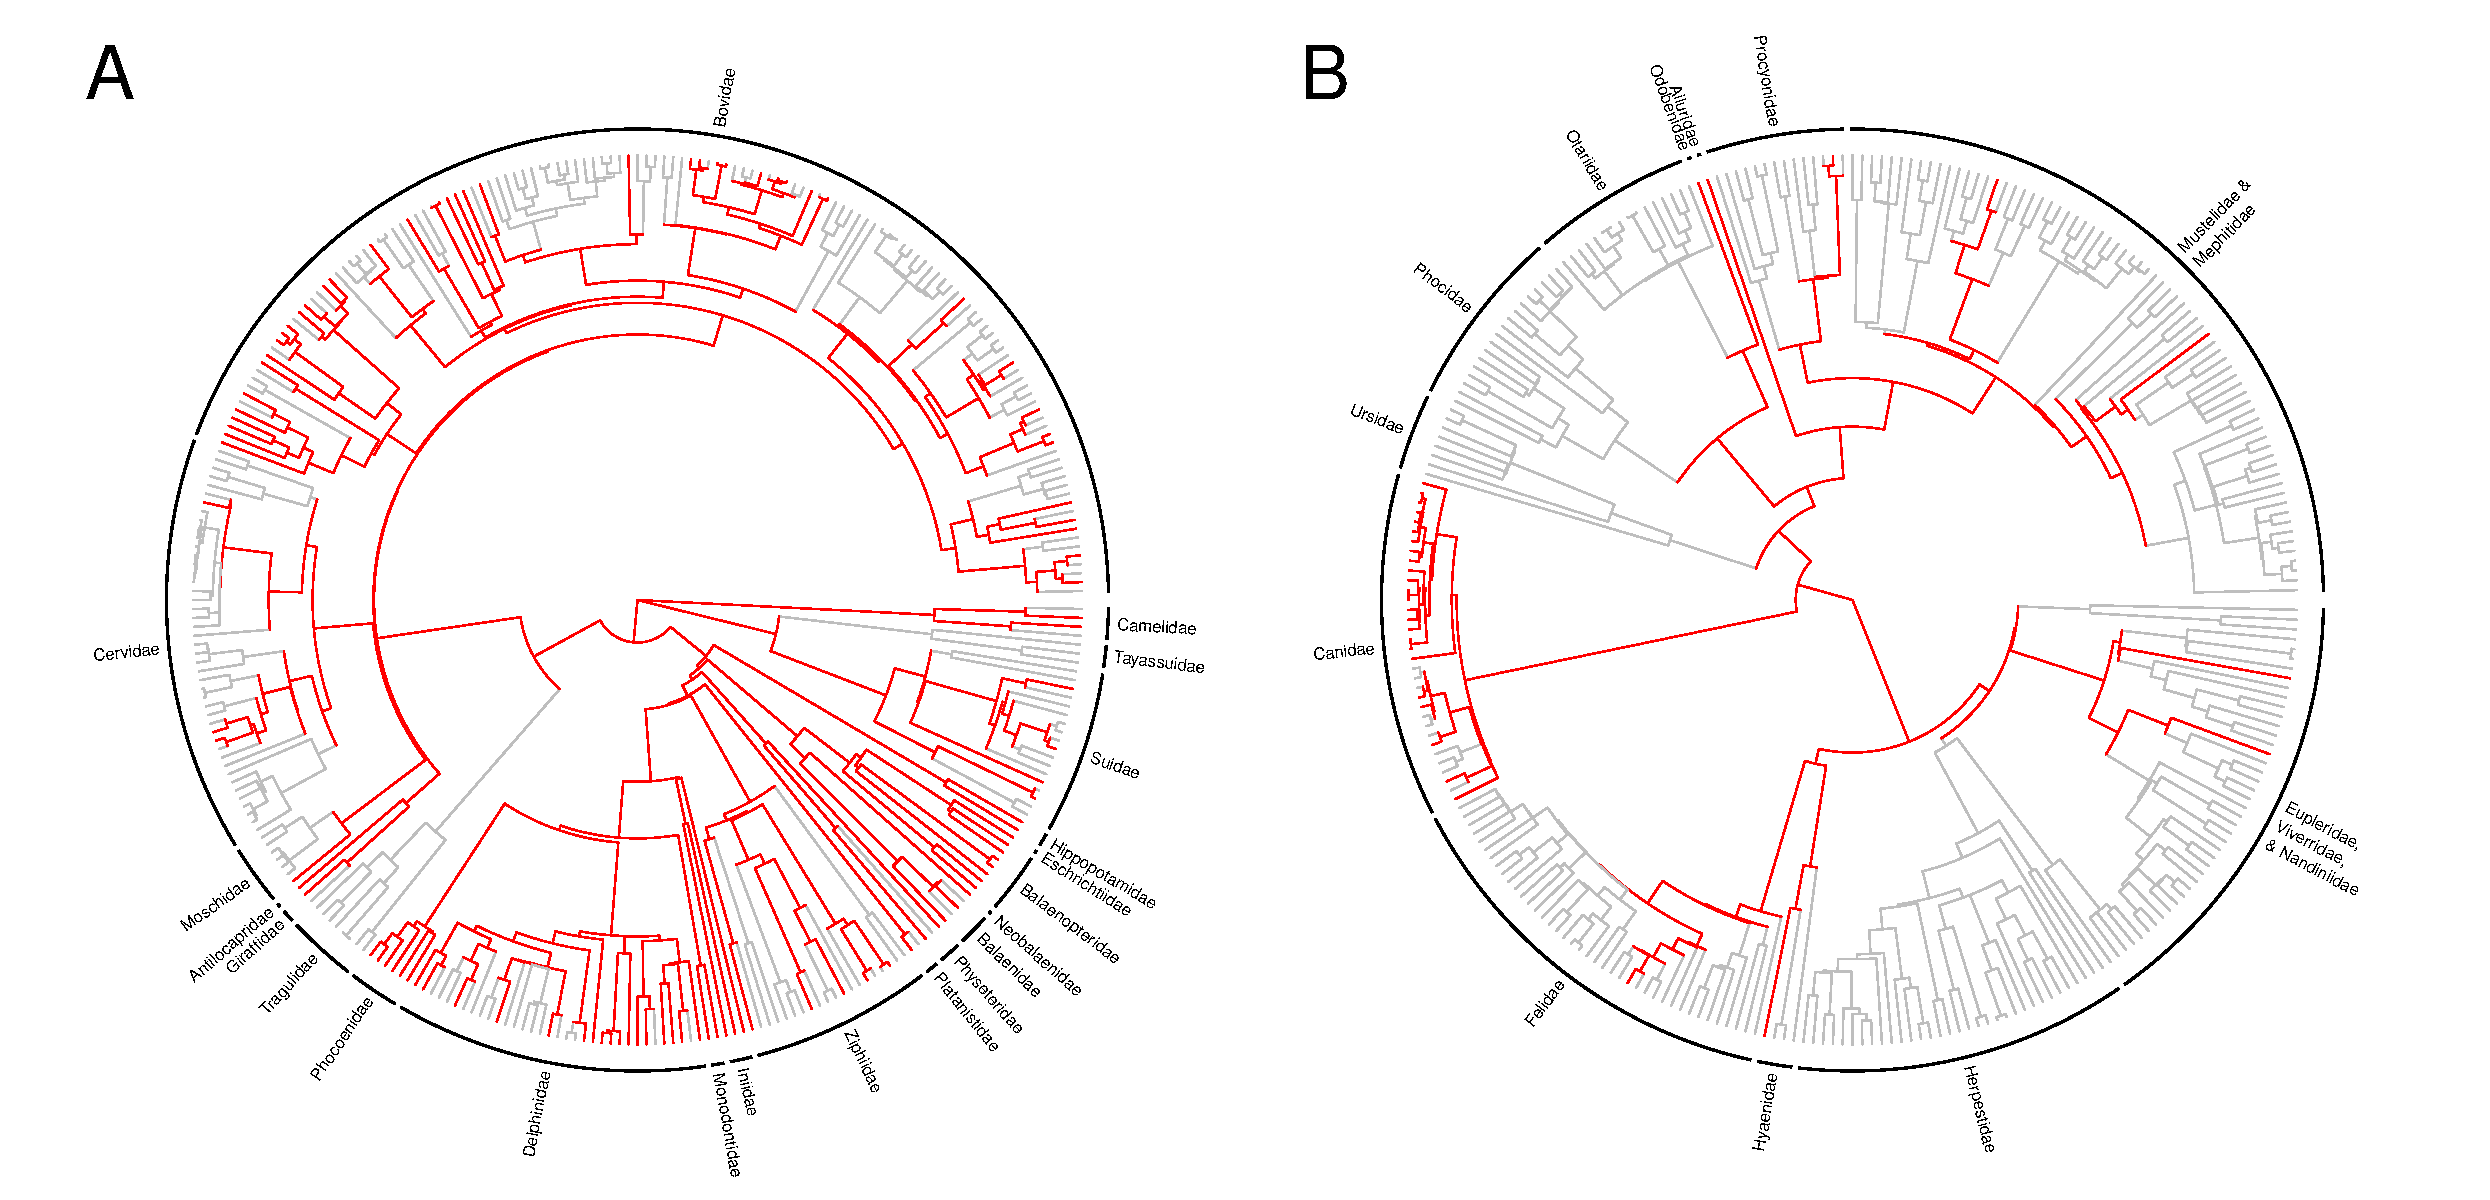
\includegraphics[width=1\textwidth]{example_coverage.pdf}
\caption{Phylogenetic distribution of available cladistic data across two mammalian orders (A: Cetartiodactyla; B: Carnivora).
Edges are colored in grey when no cladistic data is available or in red when data is available.}
\label{Figure_example_coverage}
\end{figure}
% NC: Can we change the colours, red sucks. Otherwise I like the figure a lot.
% TG: Again, will fix in the final version.

%---------------------------------------------
%
%       DISCUSSION
%
%---------------------------------------------

\section{Discussion}
Our results show that although phylogenetic relationships among living mammals are well-resolved \citep[e.g.][]{FritzTree,meredithimpacts2011,May-Collado-PeerJ}, most of the data used to build these phylogenies is molecular, and very little cladistic data is available for living mammals compared to fossil mammals \citep[e.g.][]{O'Leary08022013,ni2013oldest}.
This has implications for building Total Evidence phylogenies containing both living and fossil mammals as without sufficient cladistic data for living species, fossil placements in these trees is very uncertain \citep{GuillermeCooper}.
However, data coverage in living mammals varies across taxonomic levels and in its phylogenetic distribution.
Higher taxonomic levels are always better sampled than lower ones and within these taxonomic levels, the available data is mostly randomly distributed across the phylogeny, apart from in Carnivora and Chiroptera.

The number of living taxa with no available cladistic data was surprisingly high at the species-level: @24 out of @28 orders have a ``high'' coverage of taxa with available cladistic data (and two of the 28 orders are monospecific!).
This threshold of 75\% available data (``high'' coverage) represents the minimum amount of data required before missing data has a significant effect on the topology of Total Evidence trees \citep{GuillermeCooper}.
Beyond this threshold, there is considerable displacement of wildcard taxa (\textit{sensu} \citep{kearneyfragmentary2002}) and decreases in clade conservation \citep{GuillermeCooper}.
Therefore we expect a high probability of topological artefacts for the placement of fossil taxa at the species-level in most mammalian orders.
However, data coverage seems to be less of an issue at higher taxonomic levels (i.e. genus- and family-level).
This point is important to consider from a practical point of view because of the slight discrepancy between the neontological and the palaeontological concept of species.
While neontological species are described on accurately measured morphology, genetic distance, spatial distribution and even behaviour \citep[e.g.][]{kellymolecular2014}, palaeontological data can be based only on morphological, spatial and temporal data \citep[e.g.][]{ni2013oldest}.
Because of this difference between neontological species (\textit{sensu} reproductive isolates) and paleontological species (\textit{sensu} morpho-species %or "morphological clusters"?
), most palaeontological studies are using the genus level for their smallest OTU \citep[e.g.][]{ni2013oldest,O'Leary08022013}.
In this frame of palaeontological data usage, the data availability at the genus-level in living mammals should be our priority concern.

Regardless the low level of available data, it is encouraging that for most orders (except Carnivora and Chiroptera), data is randomly distributed across the phylogeny.
There are three different scenarii, regarding the distribution of the available data, for predicting how fossils can branch in relation to living taxa.
When only few data is available, the ideal scenario will be that it is over-dispersed (i.e. that there is data in at least every sub-clade) in order to maximize the possibilities of the fossil to branch in the right clade.
In the second scenario, when the data is randomly distributed we expected no special bias in the placement of the fossil \citep{GuillermeCooper}.
However, in the third scenario, when the data is clustered we expect two major biases to occur: (1) first, the fossil will not be able to branch within a clade containing no data (e.g. Herpestidae in Carnivora; Figure \ref{Figure_missing_data_problem} and \ref{Figure_example_coverage}B), and (2) second, the fossil will have a higher probability, at random, to branch within the clade containing most of the available data (e.g. a Carnivora fossil will have more chance to branch, randomly, to the Canidae clade than any other clade in Carnivora; Figure \ref{Figure_example_coverage}-B).
This means that fossils with uncertain phylogentic affinities (\textit{Incertae sedis}) will have a higher probability of branching by chance within the most sampled clade.

%For example in Carnivora, their is no available data for Herpestidae, therefore any fossil Herpestidae will not be able to be correctly placed in the phylogeny (figure ~\ref{Figure_example_coverage}-B.
%On the other hand, any Carnivora fossil with uncertain phylogenetic affinities (\textit{Incertae sedis} will have a higher probability of branching by chance within the Canidae because they are oversampled within the Carnivora (figure ~\ref{Figure_example_coverage}-B.

%Caveats
In this study, we treated all cladistic matrices as equal in a similar way to molecular matrices. 
For example, if matrix A contained 100 characters for taxa X and Y, and matrix B contained 50 different characters for taxa X and Z, we assumed that both matrices can be combined in a supermatrix containing 150 independent characters for taxon X, 100 for taxon Y and 50 for taxon Z.
Unfortunately, cladistic data cannot always be treated in this way because some characters may overlap.
For example, if matrix A has a character coding for the shape of a particular morphological feature and matrix B has a character coding for the presence of this morphological feature and a second character coding for its shape then these three characters are non-independent compound characters \citep{Brazeau2011}.
However, in reasonably sized matrices (\textgreater 100 characters; \citealp{GuillermeCooper,harrisonamong-character2014}) it is more likely that a number of characters are consistently conserved among the different matrices (e.g. within the Primate literature, the character \textit{p7} - the size of the $4^{th}$ lower premolar paraconid - has been used consistently for \textgreater 15 years; \citealp[e.g.][]{ross1998phylogenetic,seiffert2003fossil,marivaux2005anthropoid,seiffert2005basal,bloch2007new,kay2008anatomy,silcox2008biogeographic,seiffert2009convergent,tabuce2009anthropoid,boyer2010astragalar,seiffert2010fossil,marivaux2013djebelemur,ni2013oldest}). % NC: Remove some of these
A conservative approach to avoid compound characters would be to select only the most recent matrix for each group, but this would result in the loss of a lot of data.

%Let's code some data
Following the recommendations in \citep{GuillermeCooper}, to improve the accuracy of the topology of Total Evidence trees containing both living and fossil taxa, one should code cladistic characters for as many living species possible. 
Since the data for living mammals is usually easily available in world wide vast natural history collections, we propose that an increased effort in coding morphological characters from living species should be done via engaging in collaborative data collection projects through web portals such as \textit{Morphobank} \citep{morphobank}.

%Biology letters various stuff
\section{Ethics statement}
\section{Data accessibility statement}
All data and analysis code is available on GitHub.
\section{Authors' Contributions}
T.G. and N.C conceived and designed the experiments. T.G. performed the experiments and analysed the data. T.G. and N.C. contributed to the writing of the manuscript. All authors approved the final version of the manuscript.
\section{Competing Interests}
We have no competing interests.
\section{Acknowledgements}
David Bapst, Graeme Lloyd, Nick Matzke and April Wright.
\section{Funding statement}
This work was funded by a European Commission CORDIS Seventh Framework Programme (FP7) Marie Curie CIG grant (proposal number: 321696).

\bibliographystyle{sysbio}
\bibliography{References}

%\section{SOM}
\newcommand{\beginsupplement}{%
    \setcounter{table}{0}
    \renewcommand{\thetable}{S\arabic{table}}%
    \setcounter{figure}{0}
    \renewcommand{\thefigure}{S\arabic{figure}}%
}
\beginsupplement
%
\noindent{\Large \bf Supplementary Material}

\bigskip

\section{Data collection}
1- Data collection: key words, clade (ordinal) metacharacters, Google Search terms, Google Search protocol, Google Search rarefaction curve.

\subsection{Public repositories}
We downloaded available matrices containing fossil and/or living mammal taxa from the three following data bases using the following list of keywords:

\texttt{Mammalia; Monotremata; Marsupialia; Placentalia; Macroscelidea; Afrosoricida; Tubulidentata; Hyracoidea; Proboscidea; Sirenia; Pilosa; Cingulata; Scandentia; Dermoptera; Primates; Lagomorpha; Rodentia; Erinaceomorpha; Soricomorpha; Cetacea; Artiodactyla; Cetartiodactyla; Chiroptera; Perissodactyla; Pholidota; Carnivora; Didelphimorphia; Paucituberculata; Microbiotheria; Dasyuromorphia; Peramelemorphia; Notoryctemorphia; Diprotodontia}.

Details about each public repository specific search option is listed below. Note that some matrices have been downloaded from more than one database but that it is not an issue since we are interested in the total number of living OTUs and that if some where present in more than one matrix, they still only counted as a unique OTU.

\subsubsection{Morphobank}
We accessed the Morphobank repository (\texttt{http://www.morphobank.org/}) on the 5th of December 2014 and used the keywords listed above in the search menue. We downloaded the data associated with each project matching with the keyword.

\subsubsection{Graeme Lloyd}
We accessed Graeme Lloyd's website repository (\texttt{http://graemetlloyd.com/}) on the 5th of December 2014 and downloaded all the matrices that were available with a direct download link in the mammal data section of the website (\texttt{http://graemetlloyd.com/matrmamm.html}).

\subsubsection{Ross Mounce}
We accessed Ross Mounce's GitHub repository (\texttt{https://github.com/rossmounce}) on the 2nd of December 2014 and downloaded every 601 matrix. We then ran a shell script to select only the matrices that had any text element that match with one of the search terms. To make the matrix selection more thorough, we ignored the keywords case as well as the latin suffix (\textit{ia}, \textit{ata}, \textit{ea}, and \textit{a}).

\subsection{Google scholars}
To make sure we didn't miss any extra matrix that wasn't available on one of these repository, we ran a Google Scholar search on the 5th of January. We used the following key words:

\texttt{\textit{order} ("morphology" OR "morphological" OR "cladistic") AND characters matrix paleontology phylogeny}

were \textit{order} was replaced by all the keywords listed above. For each 33 keywords, we selected the 20 first papers to match the Google search published since 2010 resulting in 660 papers. Among these papers, not all contained relevant data (discrete morphological characters AND mammalian data). We selected only the 20 first results per search term to avoid downloading articles that were to irrelevant. Among the 660 papers, only 50 contained a total of 425 extra living OTUs (figure ~\ref{Supp_figure_google_searches}).
Also we decided to select only the articles published since 2010 because nearly every one of the recent published matrix contains both a fraction of morphological characters and OTUs from previous studies. For example in primates the character \textit{p7} coded first by \cite{ross1998phylogenetic} is reused with the same living species in \cite{seiffert2003fossil}, \cite{marivaux2005anthropoid}, \cite{seiffert2005basal}, \cite{bloch2007new}, \cite{bloch2007new}, \cite{kay2008anatomy}, \cite{silcox2008biogeographic}, \cite{seiffert2009convergent}, \cite{tabuce2009anthropoid}, \cite{boyer2010astragalar}, \cite{seiffert2010fossil}, \cite{marivaux2013djebelemur} and \cite{ni2013oldest}.

\begin{figure}[!htbp]
\centering
    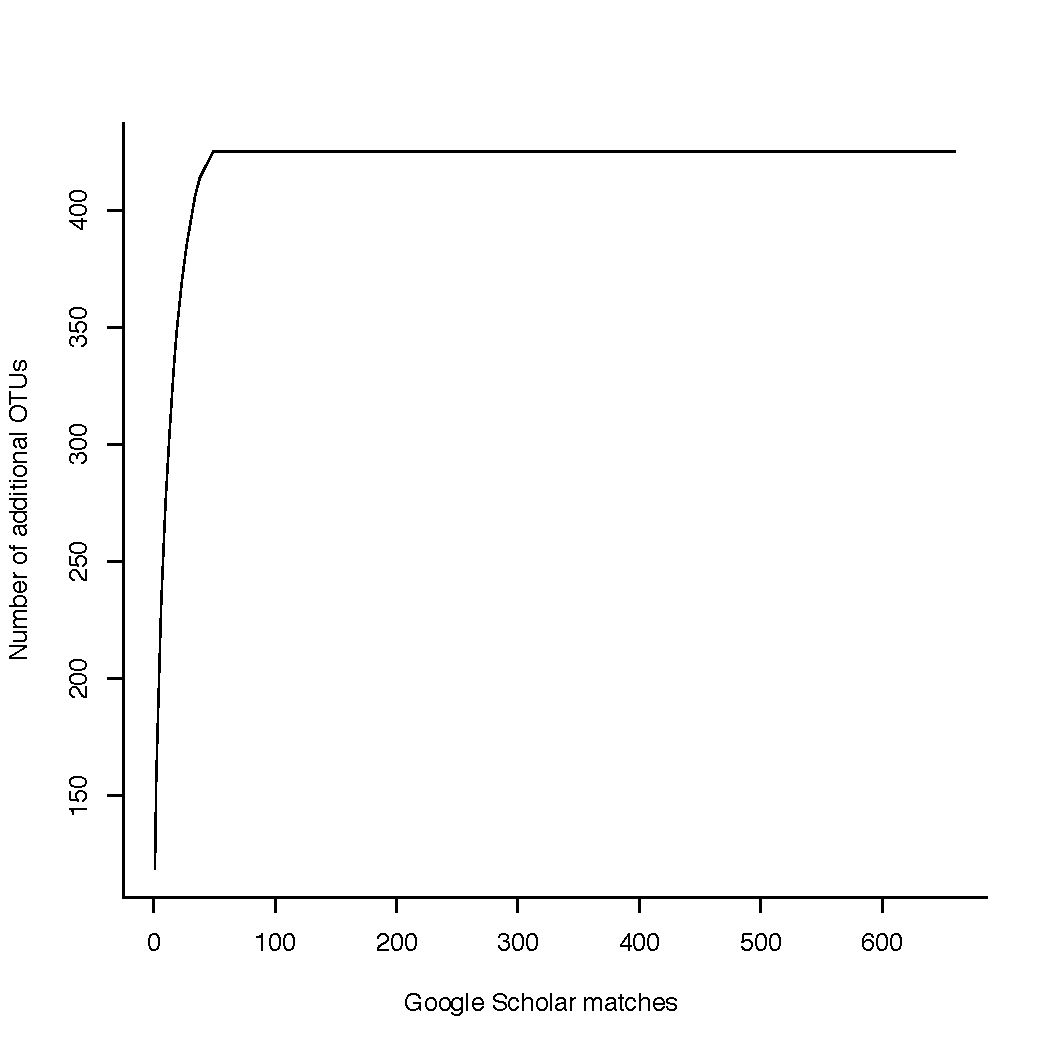
\includegraphics[width=1\textwidth]{Supplementary/Supp_figure_google_searches.pdf}
\caption{Google searches additional OTUs rarefaction curve. The x axis represent the number of google scholar matches (papers, books or abstracts) and the y axis represents the cumulative number of additional living OTUs per google scholar match.}
\label{Supp_figure_google_searches}
\end{figure}

\subsection{Standardising the matrices}
We transformed all the non-nexus matrices (tnt, word, excel, jpeg) to nexus format manually. We then cleaned the nexus matrices by removing any extra information (trees, continuous characters, morphological characters description, molecular data) to end up with nexus matrices containing only the discrete morphological data. We then manually fixed the wrong bionomial names format (e.g. \textit{H. sapiens}) into the correct ones (e.g. \textit{Homo sapiens}) using the abbreviation list in the concerned publications. 

\subsection{Selecting the living OTUs}
Finally we applied a taxonomic matching algorithm to classify the OTUs as either living or fossil. The algorithm is matching every OTU name from every matrix with one of the following taxonomic references: the list of taxa from the Fritz \textit{et al.} supertree (2009) \cite{FritzTree}; the taxonomic list from the Wilson and Reeder's Mammals Species of the World (2005) \cite{wilson2005mammal} and the list of all the mammal fossil from the Paleobio Database (\texttt{http://paleobiodb.org/cgi-bin/bridge.pl?a=login}) accessed on the 13th of Janurary 2015. The OTUs that matched with one of the two first references were considered as living OTUs, the OTUs matching with the third reference were considered as fossil OTUs, finally, the OTUs matching with non of the references were discarded (figure ~\ref{Supp_figure_Taxonomic_algorithm}).

\begin{figure}[!htbp]
\centering
    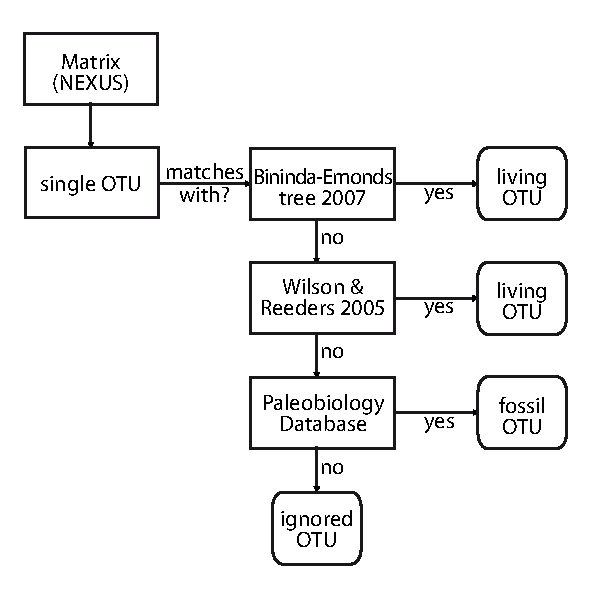
\includegraphics[width=1\textwidth]{Supplementary/Supp_figure_Taxonomic_algorithm.pdf}
\caption{Taxonomic matching algorithm used in this study. For each matrix, each operational taxonomic units (OTU) is matched with the super tree from Fritz 2009. If the OTU matches, then it is classified as living. Else it is matched with the Wilson \& Reeders 2005 taxonomy list. If the OTU matches, then it is classified as living. Else it is matched with the Paleo Database list of mammals. If the OTU matches, then it is classified as fossil. Else it is ignored.}
\label{Supp_figure_Taxonomic_algorithm}
\end{figure}

\bibliographystyle{vancouver}
\bibliography{Supp_References}


\section{Data structure}
%Tables
%Figures

\section{Supplementary results}



%END
\end{document}
